\chapter{Dynaaminen ohjelmointi}

Dynaaminen ohjelmointi on algoritmisuunnittelun tekniikka,
jota voi käyttää kahdenlaisissa tilanteissa:

\begin{itemize}
\item \textbf{Optimiratkaisun etsiminen}: Haluamme etsiä ratkaisun,
joka on jollain tavalla suurin tai pienin.
\item \textbf{Ratkaisumäärän laskeminen}: Haluamme laskea,
montako erilaista ratkaisua on olemassa.
\end{itemize}

Ideana on muotoilla laskentatehtävä
rekursiivisesti niin, että voimme ratkaista tehtävän
ratkaisemalla ensin osatehtävinä saman tehtävän pienempiä tapauksia.
Aina kun olemme ratkaisseet tietyn osatehtävän,
kirjaamme sen ratkaisun muistiin, minkä ansiosta
pystymme hakemaan ratkaisun tehokkaasti uudelleen,
jos tarvitsemme sitä myöhemmin.

Tässä luvussa tutustumme ensin dynaamisen ohjelmoinnin perusteisiin
käyttäen esimerkkinä tehtävää, jossa haluamme jakaa annetun
rahamäärän kolikoiksi.
Tämän jälkeen käymme läpi joukon muita tehtäviä, jotka esittelevät
dynaamisen ohjelmoinnin mahdollisuuksia.

\section{Perustekniikat}

Ensimmäinen esimerkkitehtävämme on seuraava:
Meillä on joukko kolikoita sekä rahamäärä,
jonka haluamme jakaa kolikoiksi.
Voimme käyttää jokaista kolikkoa miten tahansa
monta kertaa ratkaisussa.
Esimerkiksi jos kolikot ovat $\{1,3,4\}$
ja rahamäärä on $5$, yksi mahdollinen
jakotapa on $1+1+3=5$.
Haluamme selvittää vastauksen kahteen kysymykseen:

\begin{itemize}
\item \textbf{Optimiratkaisun etsiminen}:
Mikä on pienin määrä kolikoita, joilla voimme muodostaa rahamäärän?
\item \textbf{Ratkaisumäärän laskeminen}:
Monellako eri tavalla voimme muodostaa rahamäärän kolikoista?
\end{itemize}

Yllä olevassa esimerkissä pienin määrä kolikoita on 2,
koska voimme tehdä jaon $1+4=5$. Erilaisia ratkaisuja taas on 6:

\begin{multicols}{2}
\begin{itemize}
\item $1+1+1+1+1=5$
\item $1+1+3=5$
\item $1+3+1=5$
\item $3+1+1=5$
\item $1+4=5$
\item $4+1=5$
\end{itemize}
\end{multicols}

Osoittautuu, että molemmat kysymykset ratkeavat tehokkaasti
dynaamisella ohjelmoinnilla
etsimällä niille sopiva rekursiivinen esitys.

\subsection{Optimiratkaisun etsiminen}

Haluamme selvittää ensin, mikä on pienin määrä
kolikoita, joilla voimme muodostaa annetun rahamäärän.
Tätä varten määrittelemme funktion $\texttt{pienin}(x)$,
joka antaa pienimmän määrän kolikoita, joilla voimme
muodostaa rahamäärän $x$.
Esimerkiksi kun kolikot ovat $\{1,3,4\}$,
niin $\texttt{pienin}(5)=2$, mikä vastaa ratkaisua $1+4=5$.

Jotta voimme käyttää dynaamista ohjelmointia,
meidän täytyy pystyä laskemaan funktion \texttt{pienin}
arvo rekursiivisesti kutsumalla sitä itseään.
Pohjatapauksena on $\texttt{pienin}(0)=0$, koska voimme
muodostaa rahamäärän 0 käyttämättä yhtään kolikkoa.
Lisäksi on hyödyllistä määritellä $\texttt{pienin}(x)=\infty$,
kun $x<0$. Tämä tarkoittaa, että ei ole sallittua muodostaa
ratkaisua, jossa rahamäärä olisi ääretön.

Kuinka voimme sitten laskea arvon $\texttt{pienin}(x)$,
missä $x>0$? Nyt on kätevää tarkastella \emph{viimeistä}
kolikkoa, joka kuuluu ratkaisuun.
Esimerkiksi jos kolikot ovat $\{1,3,4\}$, viimeinen kolikko
on joko 1, 3 tai 4.
Jos viimeinen kolikko on 1, meidän tulee muodostaa vielä
rahamäärä $x-1$, mihin kuluu $\texttt{pienin}(x-1)$ kolikkoa.
Vastaavasti jos viimeinen kolikko on 3 tai 4,
meidän tulee muodostaa rahamäärä $x-3$ tai $x-4$.
Niinpä saamme seuraavan rekursiivisen kaavan tapaukseen $x>0$:
\[
\texttt{pienin}(x) =
    \min(\texttt{pienin}(x-1),\texttt{pienin}(x-3),\texttt{pienin}(x-4))
\]
Tässä tapauksessa funktion \texttt{pienin} ensimmäiset arvot ovat:

\begin{center}
\begin{tabular}{rrrrrrrrrrrr}
$x$ & 0 & 1 & 2 & 3 & 4 & 5 & 6 & 7 & 8 & 9 & 10 \\
\hline
$\texttt{pienin}(x)$ & 0 & 1 & 2 & 1 & 1 & 2 & 2 & 2 & 2 & 3 & 3 \\
\end{tabular}
\end{center}


Tarkastellaan sitten yleistä tilannetta, jossa meillä on $k$ kolikkoa,
joiden arvot ovat $\{c_0,c_1,\ldots,c_{k-1}\}$.
Nyt voimme jälleen muodostaa rekursiivisen kaavan samalla idealla:
\[
\texttt{pienin}(x) =
    \min(\texttt{pienin}(x-c_0),\texttt{pienin}(x-c_1),\dots,\texttt{pienin}(x-c_{k-1}))
\]

Nyt meillä on koossa kaikki ainekset tehtävän ratkaisemiseen,
ja voimme käyttää tehtävän rekursiivista muotoilua ohjelmoinnissa
seuraavasti:

\begin{code}
int pienin(int x) {
    if (x == 0) return 0;
    if (x < 0) return INF;
    int p = INF;
    for (int i = 0; i < k; i++) {
        p = min(p,pienin(x-c[i])+1);
    }
    return p;
}
\end{code}

Tässä toteutuksessa \texttt{INF} on suuri luku, joka kuvastaa ääretöntä.
Käytän\-nössä luku voisi olla esimerkiksi $10^9$,
joka on varmasti kelvollinen yläraja kolikoiden määrälle.

Ainoa ongelma yllä olevassa ratkaisussa on,
että se ei ole vielä tehokas.
Syynä tähän on, että suuren arvon $x$ käsittelyssä
funktiota \texttt{pienin} kutsutaan lukuisia kertoja
pienempien osatehtävien ratkomisessa.
Nyt kuvaan astuukin dynaamisen ohjelmoinnin keskeinen idea:
tallennamme funktion arvoja muistiin niin, että meidän
tarvitsee laskea jokainen arvo vain kerran.
Tätä varten tarvitsemme seuraavat taulukot:

\begin{code}
boolean laskettu[];
int muisti[];
\end{code}

Taulukko \texttt{laskettu} kertoo meille, onko funktion arvo
tietyllä parametrilla laskettu jo muistiin.
Jos on, taulukko \texttt{muisti} kertoo, mikä arvo on.
Nyt voimme muuttaa funktion toteutusta seuraavasti:

\begin{code}
int pienin(int x) {
    if (x == 0) return 0;
    if (x < 0) return INF;
    if (laskettu[x]) return muisti[x];
    int p = INF;
    for (int i = 0; i < k; i++) {
        p = min(p,pienin(x-c[i])+1);
    }
    laskettu[x] = true;
    muisti[x] = p;
    return p;
}
\end{code}

Funktio toimii kuten ennenkin, mutta ennen rekursiivisia kutsuja
funktio tarkastaa, onko sen arvo parametrilla $x$ jo laskettu.
Jos on, funktio palauttaa tämän arvon suoraan.
Muussa tapauksessa funktio laskee arvon rekursiivisesti
ja merkitsee sitten taulukoihin, että arvo on laskettu.

Tämän muutoksen ansiosta funktio toimii tehokkaasti,
koska jokainen funktion arvo täytyy laskea rekursiivisesti vain kerran
ja myöhemmillä kerroilla arvon saa suoraan taulukosta.
Saamme laskettua vastauksen rahamäärälle $n$ ajassa $O(nk)$,
koska jokaisessa osatehtävässä
$x=1,2,\ldots,n$ meidän täytyy käydä kerran rekursiivisesti läpi
kaikki $k$ kolikkoa.

\subsection{Ratkaisumäärän laskeminen}

Seuraavaksi haluamme laskea, montako erilaista ratkaisua
tehtävään on olemassa.
Tätä varten määrittelemme uuden funktion $\texttt{maara}(x)$,
joka kertoo, monellako tavalla voimme muodostaa rahamäärän $x$.
Esimerkiksi kun kolikot ovat $\{1,3,4\}$, niin $\texttt{maara}(5)=6$.

Tässä tapauksessa ensinnäkin $\texttt{maara}(0)=1$, koska on yksi tapa
muodostaa rahamäärä $0$: emme ota mukaan mitään kolikoita.
Sitten $\texttt{maara}(x)=0$, jos $x<0$,
koska ei ole mitään tapaa muodostaa negatiivista rahamäärää.
Rekursiivisessa tapauksessa $x>0$ laskemme yhteen kaikki
tavat, miten voimme poistaa viimeisen kolikon:
\[
\texttt{maara}(x) =
    \texttt{maara}(x-c_0)+\texttt{maara}(x-c_1)+\dots+\texttt{maara}(x-c_{k-1})
\]
Esimerkiksi kolikoiden $\{1,3,4\}$ tapauksessa saamme laskettua
arvon $\texttt{maara}(5)$ kaavalla
\[
\texttt{maara}(5) =
    \texttt{maara}(4)+\texttt{maara}(2)+\texttt{maara}(1).
\]

Seuraava metodi toteuttaa laskennan rahamäärälle $n$
tehokkaasti dynaamisella ohjelmoinnilla ajassa $O(nk)$:

\begin{code}
int maara(int x) {
    if (x == 0) return 1;
    if (x < 0) return 0;
    if (laskettu[x]) return muisti[x];
    int m = 0;
    for (int i = 0; i < k; i++) {
        m += maara(x-c[i]);
    }
    laskettu[x] = true;
    muisti[x] = m;
    return m;
}
\end{code}

\subsection{Iteratiivinen toteutus}

Dynaamisen ohjelmoinnin laskennan voi toteuttaa myös iteratiivisesti
ilman rekursiota.
Tällaisessa toteutuksessa laskemme funktion arvot taulukkoon
pienimmästä arvosta suurimpaan.
Esimerkiksi voimme laskea seuraavasti, monellako tavalla
voimme muodostaa rahamäärän $n$:

\begin{code}
int maara(int n) {
    muisti[0] = 1;
    for (int i = 1; i <= n; i++) {
        muisti[i] = 0;
        for (int j = 0; j < k; j++) {
            if (i-c[j] >= 0) {
                muisti[i] += muisti[i-c[j]];
            }
        }
    }
    return muisti[n];
}
\end{code}

Tämä ratkaisu vie aikaa $O(nk)$, eli se on yhtä nopea kuin
rekursiivinen versio.
Ratkaisun etuna on, että se on hieman lyhyempi kirjoittaa
kuin rekursiivinen ratkaisu.

\section{Esimerkkejä}

Nyt olemme käyneet läpi dynaamisen ohjelmoinnin perustekniikat
ja on aika ottaa käsittelyyn lisää tehtäviä,
jotka opettavat meille lisää dynaamisesta ohjelmoinnista.

Dynaamista ohjelmointia voi käyttää aina silloin,
kun voimme esittää tilanteen rekursiivisena funktiona,
jonka eri parametrien määrä on niin pieni, että voimme
tallentaa muistiin funktion arvot kaikilla parametreilla.
Vaikeutena on usein keksiä, mikä on hyvä rekursiivinen
muotoilu tehtävälle.

\subsection{Pisin nouseva alijono}

Ensimmäinen tehtävämme on laskea, kuinka pitkä on
$n$ lukua sisältävän taulukon \emph{pisin nouseva alijono}.
Tämä tarkoittaa, että meidän tulee valita taulukosta
mahdollisimman pitkä jono alkioita niin,
että seuraava alkio on aina edellistä suurempi.
Kuvassa \ref{fig:pisnou} on esimerkki taulukosta,
jonka pisin nouseva alijono on pituudeltaan 4.

\begin{figure}
\center
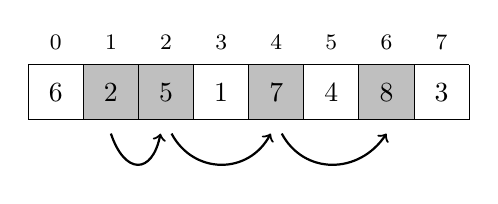
\begin{tikzpicture}[scale=0.7]
\fill[color=lightgray] (1,0) rectangle (2,1);
\fill[color=lightgray] (2,0) rectangle (3,1);
\fill[color=lightgray] (4,0) rectangle (5,1);
\fill[color=lightgray] (6,0) rectangle (7,1);
\draw (0,0) grid (8,1);
\node at (0.5,0.5) {$6$};
\node at (1.5,0.5) {$2$};
\node at (2.5,0.5) {$5$};
\node at (3.5,0.5) {$1$};
\node at (4.5,0.5) {$7$};
\node at (5.5,0.5) {$4$};
\node at (6.5,0.5) {$8$};
\node at (7.5,0.5) {$3$};
\draw[thick,->] (1.5,-0.25) .. controls (1.75,-1.00) and (2.25,-1.00) .. (2.4,-0.25);
\draw[thick,->] (2.6,-0.25) .. controls (3.0,-1.00) and (4.0,-1.00) .. (4.4,-0.25);
\draw[thick,->] (4.6,-0.25) .. controls (5.0,-1.00) and (6.0,-1.00) .. (6.5,-0.25);
\footnotesize
\node at (0.5,1.4) {$0$};
\node at (1.5,1.4) {$1$};
\node at (2.5,1.4) {$2$};
\node at (3.5,1.4) {$3$};
\node at (4.5,1.4) {$4$};
\node at (5.5,1.4) {$5$};
\node at (6.5,1.4) {$6$};
\node at (7.5,1.4) {$7$};
\end{tikzpicture}
\caption{Taulukon pisin nouseva alijono on $[2,5,7,8]$.}
\label{fig:pisnou}
\end{figure}

Voimme lähestyä tehtävää laskemalla jokaiselle taulukon
kohdalle $x=0,1,\dots,n-1$ arvon $\texttt{pisin}(x)$:
kuinka pitkä on pisin nouseva alijono, joka päättyy tähän kohtaan.
Kun olemme laskeneet kaikki nämä arvot, suurin arvoista kertoo,
kuinka pitkä on pisin nouseva alijono koko taulukossa.
Esimerkiksi kuvan \ref{fig:pisnou} taulukossa $\texttt{pisin}(6)=4$,
koska kohdassa $6$ pisin nouseva alijono on pituudeltaan $4$.

Millainen on sitten pisin kohtaan $x$ päättyvä alijono?
Yksi mahdollisuus on, että alijonossa on vain yksi alkio,
jolloin $\texttt{pisin}(x)=1$.
Jos kuitenkin alijonossa on useampia alkioita,
voimme käydä läpi vaihtoehdot, missä kohdassa on alijonon
toiseksi viimeinen alkio.
Meidän täytyy siis tarkastella kohtia $k$, joille pätee $k<x$
ja joiden alkiot ovat pienempiä kuin kohdan $x$ alkio.
Jokaisessa tällaisessa tapauksessa voimme muodostaa alijonon,
jossa on ensin pisin kohtaan $k$ päättyvä alijono ja
sitten vielä kohdan $x$ alkio.
Tuloksena olevan alijonon pituus on $\texttt{pituus}(k)+1$.
Jokin tällainen alijono on varmasti pisin kohtaan $x$ päättyvä alijono.

Seuraava koodi laskee jokaiseen kohtaan $x=0,1,\dots,n-1$
pisimmän kohtaan päättyvän alijonon pituuden yllä kuvattua
ideaa käyttäen.
Koodi olettaa, että taulukon sisältö on taulukossa \texttt{taulu},
ja se muodostaa taulukon \texttt{pisin}, jossa on pisimpien
alijonojen pituudet.
Koodin suoritus vie aikaa $O(n^2)$, koska siinä on kaksi sisäkkäistä silmukkaa.

\begin{code}
for (int i = 0; i < n; i++) {
    pisin[i] = 1;
    for (int j = 0; j < i; j++) {
        if (taulu[j] < taulu[i]) {
            pisin[i] = max(pisin[i],pisin[j]+1);
        }
    }
}
\end{code}

\subsection{Repunpakkaus}

\subsection{Reitti ruudukossa}
